\documentclass{standalone}
\usepackage{tikz}
\usetikzlibrary{patterns, positioning}


\begin{document}
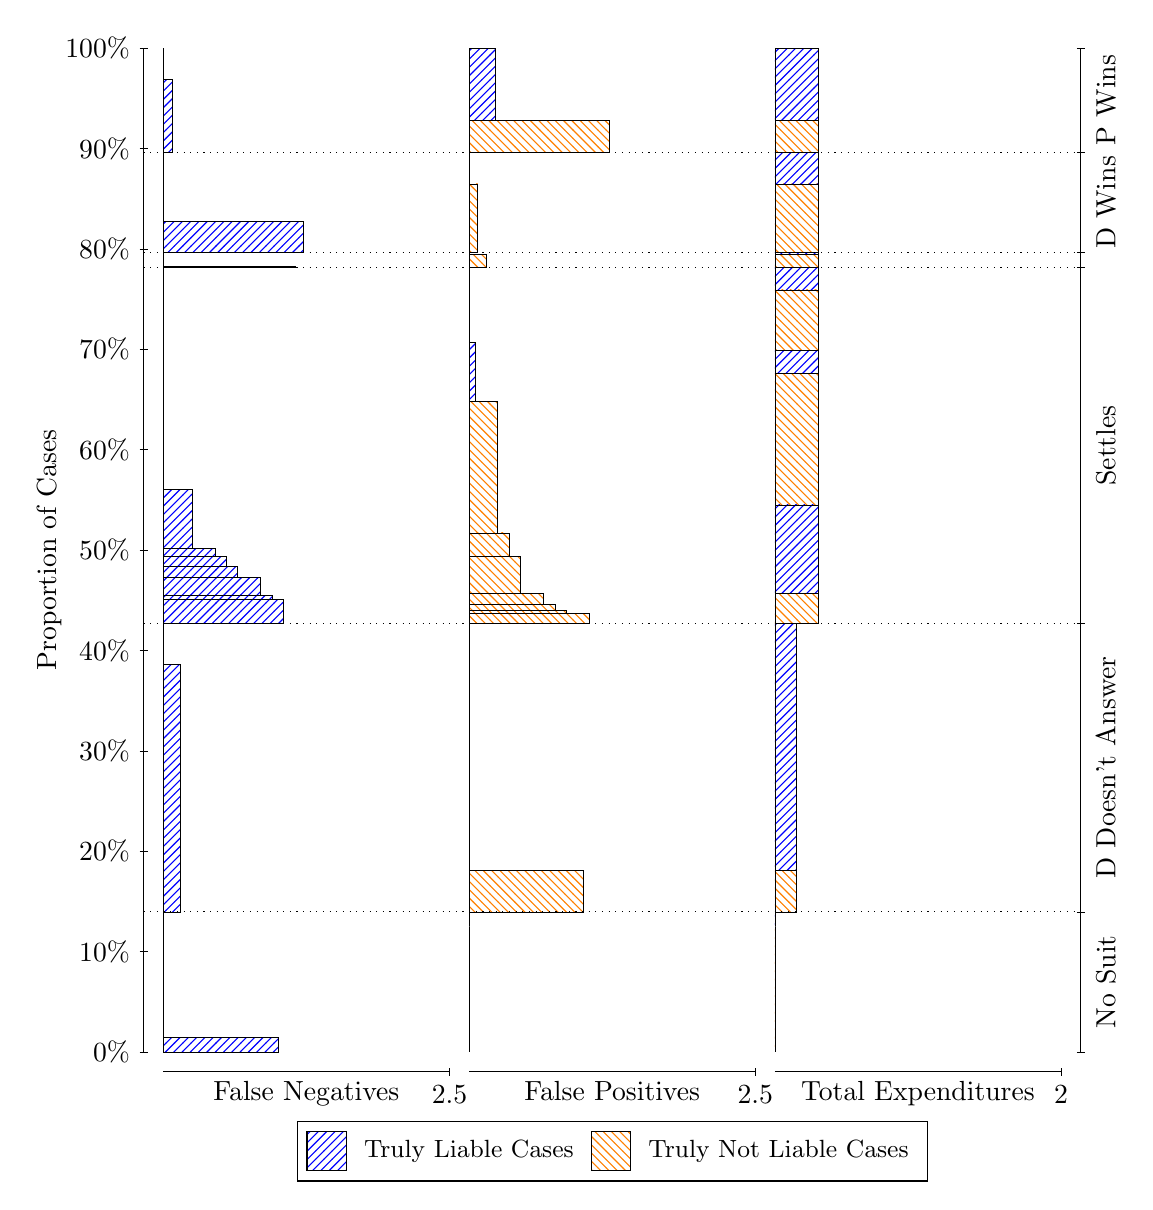
\begin{tikzpicture}
\draw[black, very thin] (1.5,1.75) -- (1.5,14.5);
\node[rotate=90, text=black, anchor=center] at (0.3, 8.125) {Proportion of Cases};
\draw[black, very thin] (1.45,1.75) -- (1.55,1.75);
\node[text=black, anchor=east] at (1.45, 1.75) {0\%};
\draw[black, very thin] (1.45,3.025) -- (1.55,3.025);
\node[text=black, anchor=east] at (1.45, 3.025) {10\%};
\draw[black, very thin] (1.45,4.3) -- (1.55,4.3);
\node[text=black, anchor=east] at (1.45, 4.3) {20\%};
\draw[black, very thin] (1.45,5.575) -- (1.55,5.575);
\node[text=black, anchor=east] at (1.45, 5.575) {30\%};
\draw[black, very thin] (1.45,6.85) -- (1.55,6.85);
\node[text=black, anchor=east] at (1.45, 6.85) {40\%};
\draw[black, very thin] (1.45,8.125) -- (1.55,8.125);
\node[text=black, anchor=east] at (1.45, 8.125) {50\%};
\draw[black, very thin] (1.45,9.4) -- (1.55,9.4);
\node[text=black, anchor=east] at (1.45, 9.4) {60\%};
\draw[black, very thin] (1.45,10.675) -- (1.55,10.675);
\node[text=black, anchor=east] at (1.45, 10.675) {70\%};
\draw[black, very thin] (1.45,11.95) -- (1.55,11.95);
\node[text=black, anchor=east] at (1.45, 11.95) {80\%};
\draw[black, very thin] (1.45,13.225) -- (1.55,13.225);
\node[text=black, anchor=east] at (1.45, 13.225) {90\%};
\draw[black, very thin] (1.45,14.5) -- (1.55,14.5);
\node[text=black, anchor=east] at (1.45, 14.5) {100\%};

\draw[black, very thin] (13.4,1.75) -- (13.4,14.5);
\draw[black, very thin] (13.35,1.75) -- (13.45,1.75);
\node[anchor=west] at (13.35, 1.75) {};
\draw[black, very thin] (13.35,3.5293) -- (13.45,3.5293);
\node[anchor=west] at (13.35, 3.5293) {};
\draw[black, very thin] (13.35,7.196) -- (13.45,7.196);
\node[anchor=west] at (13.35, 7.196) {};
\draw[black, very thin] (13.35,11.71) -- (13.45,11.71);
\node[anchor=west] at (13.35, 11.71) {};
\draw[black, very thin] (13.35,11.901) -- (13.45,11.901);
\node[anchor=west] at (13.35, 11.901) {};
\draw[black, very thin] (13.35,13.177) -- (13.45,13.177);
\node[anchor=west] at (13.35, 13.177) {};
\draw[black, very thin] (13.35,14.5) -- (13.45,14.5);
\node[anchor=west] at (13.35, 14.5) {};

\draw[black, very thin, pattern color=blue, pattern=north east lines] (1.75,1.75) rectangle (3.2033,1.9372);
\draw[black, very thin, pattern color=orange, pattern=north west lines] (1.75,1.9372) rectangle (1.75,3.5293);
\draw[black, very thin, pattern color=blue, pattern=north east lines] (1.75,3.5293) rectangle (1.968,6.6725);
\draw[black, very thin, pattern color=orange, pattern=north west lines] (1.75,6.6725) rectangle (1.75,7.196);
\draw[black, very thin, pattern color=blue, pattern=north east lines] (1.75,7.196) rectangle (3.276,7.494);
\draw[black, very thin, pattern color=blue, pattern=north east lines] (1.75,7.494) rectangle (3.1307,7.5453);
\draw[black, very thin, pattern color=blue, pattern=north east lines] (1.75,7.5453) rectangle (2.9853,7.7762);
\draw[black, very thin, pattern color=blue, pattern=north east lines] (1.75,7.7762) rectangle (2.6947,7.9122);
\draw[black, very thin, pattern color=blue, pattern=north east lines] (1.75,7.9122) rectangle (2.5493,8.0403);
\draw[black, very thin, pattern color=blue, pattern=north east lines] (1.75,8.0403) rectangle (2.404,8.1421);
\draw[black, very thin, pattern color=blue, pattern=north east lines] (1.75,8.1421) rectangle (2.1133,8.8968);
\draw[black, very thin, pattern color=orange, pattern=north west lines] (1.75,8.8968) rectangle (1.75,11.71);
\draw[black, very thin, pattern color=blue, pattern=north east lines] (1.75,11.71) rectangle (3.4213,11.731);
\draw[black, very thin, pattern color=orange, pattern=north west lines] (1.75,11.731) rectangle (1.75,11.901);
\draw[black, very thin, pattern color=blue, pattern=north east lines] (1.75,11.901) rectangle (3.5303,12.303);
\draw[black, very thin, pattern color=orange, pattern=north west lines] (1.75,12.303) rectangle (1.75,13.177);
\draw[black, very thin, pattern color=blue, pattern=north east lines] (1.75,13.177) rectangle (1.859,14.098);
\draw[black, very thin, pattern color=orange, pattern=north west lines] (1.75,14.098) rectangle (1.75,14.5);
\draw[black, very thin, pattern color=orange, pattern=north west lines] (5.6333,1.75) rectangle (5.6333,3.3421);
\draw[black, very thin, pattern color=blue, pattern=north east lines] (5.6333,3.3421) rectangle (5.6333,3.5293);
\draw[black, very thin, pattern color=orange, pattern=north west lines] (5.6333,3.5293) rectangle (7.0867,4.0527);
\draw[black, very thin, pattern color=blue, pattern=north east lines] (5.6333,4.0527) rectangle (5.6333,7.196);
\draw[black, very thin, pattern color=orange, pattern=north west lines] (5.6333,7.196) rectangle (7.1593,7.3154);
\draw[black, very thin, pattern color=orange, pattern=north west lines] (5.6333,7.3154) rectangle (6.8687,7.3615);
\draw[black, very thin, pattern color=orange, pattern=north west lines] (5.6333,7.3615) rectangle (6.7233,7.4339);
\draw[black, very thin, pattern color=orange, pattern=north west lines] (5.6333,7.4339) rectangle (6.578,7.5787);
\draw[black, very thin, pattern color=orange, pattern=north west lines] (5.6333,7.5787) rectangle (6.2873,8.0477);
\draw[black, very thin, pattern color=orange, pattern=north west lines] (5.6333,8.0477) rectangle (6.142,8.3416);
\draw[black, very thin, pattern color=orange, pattern=north west lines] (5.6333,8.3416) rectangle (5.9967,10.009);
\draw[black, very thin, pattern color=blue, pattern=north east lines] (5.6333,10.009) rectangle (5.706,10.764);
\draw[black, very thin, pattern color=blue, pattern=north east lines] (5.6333,10.764) rectangle (5.6333,11.71);
\draw[black, very thin, pattern color=orange, pattern=north west lines] (5.6333,11.71) rectangle (5.8513,11.88);
\draw[black, very thin, pattern color=blue, pattern=north east lines] (5.6333,11.88) rectangle (5.6333,11.901);
\draw[black, very thin, pattern color=orange, pattern=north west lines] (5.6333,11.901) rectangle (5.7423,12.775);
\draw[black, very thin, pattern color=blue, pattern=north east lines] (5.6333,12.775) rectangle (5.6333,13.177);
\draw[black, very thin, pattern color=orange, pattern=north west lines] (5.6333,13.177) rectangle (7.4137,13.579);
\draw[black, very thin, pattern color=blue, pattern=north east lines] (5.6333,13.579) rectangle (5.9603,14.5);
\draw[black, very thin, pattern color=orange, pattern=north west lines] (9.5167,1.75) rectangle (9.5167,3.3421);
\draw[black, very thin, pattern color=blue, pattern=north east lines] (9.5167,3.3421) rectangle (9.5167,3.5293);
\draw[black, very thin, pattern color=orange, pattern=north west lines] (9.5167,3.5293) rectangle (9.7892,4.0527);
\draw[black, very thin, pattern color=blue, pattern=north east lines] (9.5167,4.0527) rectangle (9.7892,7.196);
\draw[black, very thin, pattern color=orange, pattern=north west lines] (9.5167,7.196) rectangle (10.062,7.5787);
\draw[black, very thin, pattern color=blue, pattern=north east lines] (9.5167,7.5787) rectangle (10.062,8.6993);
\draw[black, very thin, pattern color=orange, pattern=north west lines] (9.5167,8.6993) rectangle (10.062,10.367);
\draw[black, very thin, pattern color=blue, pattern=north east lines] (9.5167,10.367) rectangle (10.062,10.665);
\draw[black, very thin, pattern color=orange, pattern=north west lines] (9.5167,10.665) rectangle (10.062,11.428);
\draw[black, very thin, pattern color=blue, pattern=north east lines] (9.5167,11.428) rectangle (10.062,11.71);
\draw[black, very thin, pattern color=orange, pattern=north west lines] (9.5167,11.71) rectangle (10.062,11.88);
\draw[black, very thin, pattern color=blue, pattern=north east lines] (9.5167,11.88) rectangle (10.062,11.901);
\draw[black, very thin, pattern color=orange, pattern=north west lines] (9.5167,11.901) rectangle (10.062,12.775);
\draw[black, very thin, pattern color=blue, pattern=north east lines] (9.5167,12.775) rectangle (10.062,13.177);
\draw[black, very thin, pattern color=orange, pattern=north west lines] (9.5167,13.177) rectangle (10.062,13.579);
\draw[black, very thin, pattern color=blue, pattern=north east lines] (9.5167,13.579) rectangle (10.062,14.5);
\draw[black, dotted] (1.5,3.5293) -- (13.4,3.5293);
\draw[black, dotted] (1.5,7.196) -- (13.4,7.196);
\draw[black, dotted] (1.5,11.71) -- (13.4,11.71);
\draw[black, dotted] (1.5,11.901) -- (13.4,11.901);
\draw[black, dotted] (1.5,13.177) -- (13.4,13.177);
\draw[black, very thin] (1.75,1.5) -- (5.3833,1.5);
\node[text=black, anchor=north] at (3.5667, 1.5) {False Negatives};
\draw[black, very thin] (5.3833,1.45) -- (5.3833,1.55);
\node[text=black, anchor=north] at (5.3833, 1.45) {2.5};

\draw[black, very thin] (5.6333,1.5) -- (9.2667,1.5);
\node[text=black, anchor=north] at (7.45, 1.5) {False Positives};
\draw[black, very thin] (9.2667,1.45) -- (9.2667,1.55);
\node[text=black, anchor=north] at (9.2667, 1.45) {2.5};

\draw[black, very thin] (9.5167,1.5) -- (13.15,1.5);
\node[text=black, anchor=north] at (11.333, 1.5) {Total Expenditures};
\draw[black, very thin] (13.15,1.45) -- (13.15,1.55);
\node[text=black, anchor=north] at (13.15, 1.45) {2};

\node[text=black, centered, rotate=90] at (13.72, 2.6396) {No Suit};
\node[text=black, centered, rotate=90] at (13.72, 5.3626) {D Doesn't Answer};
\node[text=black, centered, rotate=90] at (13.72, 9.4528) {Settles};

\node[text=black, centered, rotate=90] at (13.72, 12.539) {D Wins};
\node[text=black, centered, rotate=90] at (13.72, 13.839) {P Wins};

\draw (7.449999999999999,1.5) node[draw=none] (baseCoordinate) {};
\begin{scope}[align=center]
        \matrix[scale=0.5, draw=black, below=0.5cm of baseCoordinate, nodes={draw}, column sep=0.1cm]{
            \node[rectangle, draw, minimum width=0.5cm, minimum height=0.5cm, pattern color=blue, pattern=north east lines] {}; &
            \node[draw=none, font=\small, text=black] (B) {Truly Liable Cases}; &
            \node[rectangle, draw, minimum width=0.5cm, minimum height=0.5cm, pattern color=orange, pattern=north west lines] {}; &
            \node[draw=none, font=\small, text=black] (B) {Truly Not Liable Cases}; \\
            };
\end{scope}

\end{tikzpicture}
\end{document}